\documentclass{article}
\usepackage{tikz} 
\usepackage[utf8]{inputenc}
\usepackage{amsmath}
\usepackage{listings}
\usepackage{amsfonts}
\usepackage{amssymb}
\usepackage{tabularx}
\usepackage{enumitem}
\usepackage{algorithm}% http://ctan.org/pkg/algorithm
\usepackage[noend]{algpseudocode}% http://ctan.org/pkg/algorithmicx
\usepackage{tikz}
\usepackage{graphicx}
\usetikzlibrary{arrows,positioning} 
\usepackage{subcaption}
\usepackage{multicol,caption}
\usepackage{geometry}
 \geometry{
 a4paper,
 total={210mm,297mm},
 left=20mm,
 right=20mm,
 top=20mm,
 bottom=20mm,
 }

\definecolor{talk}{HTML}{729FCF}
\definecolor{talk2}{HTML}{E8A753}
\definecolor{grey}{HTML}{DBDCDD}

\pgfarrowsdeclarecombine{ring}{ring}{}{}{o}{o}
\thispagestyle{empty}
\DeclareMathOperator{\ringarrow}{\raisebox{0.5ex}{\tikz[baseline]{\draw[ring->](0,0)--(2em,0);}}}

\tikzset{
    %Define standard arrow tip
    >=stealth',
    %Define style for boxes
    observed/.style={
           rectangle,
           rounded corners,
           draw=black, thick,
           minimum width=3em,
           minimum height=1.5em,
           font=\footnotesize,
           text centered,
           fill=talk!50},
     latent/.style={	(Switch) edge (X)
           circle,
           rounded corners,
           draw=black, thick, dashed,
           minimum width=.5em,
           minimum height=.5em,
           font=\footnotesize,
           text centered,
           fill=black!10!white
           },
    % Define arrow style
    pil/.style={
           o->,
           thick,
           shorten <=2pt,
           shorten >=2pt,},
    sh/.style={ shade, shading=axis, left color=red, right color=green,
    shading angle=45 }
    
}
   
\begin{document}
\def\ci{\perp\!\!\!\perp} % from Wikipedia

\begin{enumerate}
\item D-separation still applies after intervention.
 
${(Cancer \ci Asthma|Smoke)_{G_{\overline{X}}} \implies P(Cancer|do(Smoke),Asthma) = P(Cancer|do(Smoke)}$
\item If there are no backdoor paths from $X$ to $Y$ then intervention$\equiv$observation.

${(\hat{X} \ci Cancer|X,Poverty)_{G^{\dagger}} \implies P(Cancer|do(Smoke),Poverty) = P(Cancer|Smoke,Poverty)}$
\item If there are only backdoor paths from $X$ to $Y$ then intervention doesn't change $P(Y)$.

$(\hat{X} \ci Diet)_{G^{\dagger}} \implies P(Diet|do(Smoke)) = P(Diet)$
\end{enumerate}
\begin{figure}[h]
\centering
\begin{subfigure}[t]{0.45\textwidth}
\centering
\caption{$G^{\dagger}$}
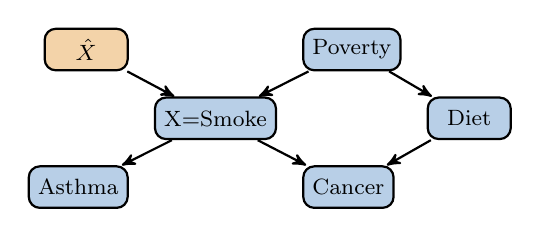
\begin{tikzpicture}[->,shorten >=0pt,shorten <=0pt,node distance=0.45cm,thick,main node/.style={observed}]
\node[main node](X){X=Smoke};
\node[main node, above right=of X](P){Poverty};
\node[main node, below right=of P](D){Diet};
\node[main node, below right=of X](C){Cancer};
\node[main node, fill=talk2!50, above left=of X](Switch){$\hat{X}$};
\node[main node, below left=of X](A){Asthma};
\path[]
	(Switch) edge (X)
	(X) edge (C)
	(D) edge (C)
	(X) edge (A)
	(P) edge (D) edge (X);
\end{tikzpicture}
\end{subfigure}
\begin{subfigure}[t]{0.45\textwidth}
\centering
\caption{$G_{\overline{X}}$}
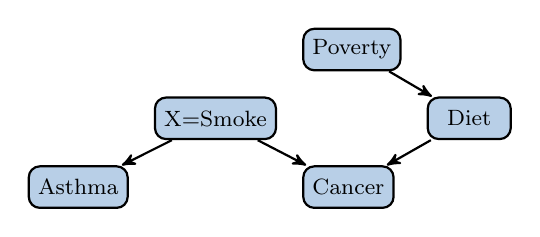
\begin{tikzpicture}[->,shorten >=0pt,shorten <=0pt,node distance=0.45cm,  thick,main node/.style={observed}, shaded/.style={latent}]
\node[main node](X){X=Smoke};
\node[main node, above right=of X](P){Poverty};
\node[main node, below right=of P](D){Diet};
\node[main node, below right=of X](C){Cancer};
\node[main node, below left=of X](A){Asthma};
\path[]
	(X) edge (C) edge (A)
	(D) edge (C)
	(P) edge (D);
\end{tikzpicture}
\end{subfigure}
\end{figure}

\end{document}